% remember to set these at the start of each chapter
\chapter{Title of Chapter 2}
\label{chapt2} 

%%%%%%%%%%%%%%%%%%
\vspace{60pt}


%%% ---------------------
%%% Publication citation 
%%% ---------------------
The content of this chapter is a second revision of the manuscript text for publication under the following citation:\\
% \vspace{20pt}

\begin{topbot}
Heider, F. (1946). Attitudes and cognitive organization. The Journal of psychology, 21(1), 107-112.
\end{topbot}

\newpage


%%% ---------------------
%%% Paper title
%%% ---------------------
\begin{center}
    \Large \textbf{Your first paper tile}
\end{center}

\vspace{40pt}

%%% ---------------------
%%% Authors
%%% ---------------------
\begin{center}
First Author\\
\textit{School of Computational Science and Engineering}\\
\textit{McMaster University, Hamilton, ON, Canada}\\
\textit{Email: \href{mailto:xxxxx@mcmaste.ca}{xxxx@mcmaste.ca}}

\vspace{10pt}

Second Author\\
\textit{DeGroote School of Business}\\
\textit{McMaster University}\\
\textit{Email: \href{mailto:xxxx@mcmaster.ca}{xxxx@mcmaster.ca}}

\end{center}


\vspace{30pt}

\begin{onehalfspacing}
%%-----------------------

\section*{\centering Abstract}
First paper abastract.


\paragraph{\textit{\textbf{Keywords:}}} \textit{keyword, keyword2} 
 


\vspace{20pt} 

\section{Section Title 2}
\label{s-1-cc}
Introduction  \citet{heider1946attitudes} 
\citep{doreian1996partitioning}

\subsection{Section Title 2}

\blindtext

\subsubsection{Section Title 3}
\blindtext 

%% FIGURE 01 -------
\begin{figure}[h]
    \centering
    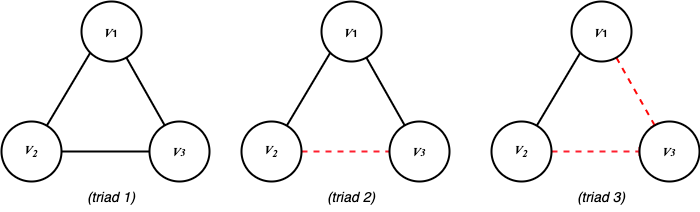
\includegraphics[width=0.75\textwidth]{Figs/Chapter2/fig_exmp.png}
    \caption{Caption.}
\label{fig:1-cc}  
\end{figure}



\end{onehalfspacing}



\bibliographystyle{dcu}
\bibliography{Bibliography}

